\documentclass{article}
\usepackage{polski}
\usepackage{listings}
\usepackage{graphicx}
\usepackage{xcolor}
\usepackage{float}
\usepackage{amsmath}
\newcommand{\bigO}{\mathcal{O}}

\lstdefinestyle{mystyle}{
    keywordstyle=\color{blue},       % kolor słów kluczowych
    numberstyle=\tiny\color{gray},   % kolor numerów linii
    basicstyle=\ttfamily\footnotesize, % styl podstawowy
    breaklines=true,                 % łamanie długich wierszy
    captionpos=b,                    % pozycja podpisu
    numbers=left,                    % numery linii po lewej stronie
    numbersep=1pt,                   % odstęp numerów linii
    showspaces=false,                % nie pokazuj spacji
    tabsize=2                        % rozmiar tabulacji
}

\renewcommand{\lstlistingname}{Kod}
\renewcommand{\figurename}{Wykres}

\title{Sprawozdanie - Lista 1}
\author{Jakub Zdancewicz}
\date{}

\begin{document}

\maketitle

\tableofcontents
\newpage

\section{Wstęp}
Sortowanie to jeden z fundamentalnych problemów informatyki, mający szerokie zastosowanie w wielu dziedzinach. Algorytmy sortowania odgrywają kluczową rolę w wielu aplikacjach, a ich wydajność istotnie wpływa na czas działania. Wybór odpowiedniego algorytmu sortującego jest zatem istotną decyzją podczas tworzenia oprogramowania. W niniejszym sprawozdaniu przeanalizujemy trzy popularne algorytmy sortowania wraz z ich wybranymi modyfikacjami:
\begin{itemize}
    \item Insertion Sort
    \item Merge Sort
    \item Heap Sort
\end{itemize}
oraz porównamy ich efektywność na zestawach danych o różnych rozmiarach, badając liczbę operacji przypisań i porównań.


\section{Opis zaimplementowanych algorytmów}
Każdy z algorytmów został przetestowany na 10 losowo wygenerowanych tablicach dla każdej z 15 wybranych długości. Elementy tablic to liczby wymierne z zakresu $[-10^6, 10^6]$. Minimalna długość tablicy wynosiła 2, a maksymalna 100000. Średnia liczba operacji przypisań i porównań dla tablic o danej długości $n$ jest wyliczana według wzoru:
\[
    L_n = \sum_{i=1}^{10} \left\lceil\frac{porownania_i}{10}\right\rceil + \left\lceil\frac{przypisania_i}{10}\right\rceil
\]
gdzie:
\begin{itemize}
    \item[] $L_n$ - średnia liczba operacji dla tablicy o długości $n$,
    \item[] $\text{porownania}_i$ - liczba porównań wykonanych dla i-tej tablicy,
    \item[] $\text{przypisania}_i$ - liczba przypisań wykonanych dla i-tej tablicy.
\end{itemize}

\newpage
\subsection{Insertion Sort}
\textit{Insertion Sort} to algorytm działający w czasie $\Theta(n^2)$. Poniżej przedstawiamy kluczowy fragment jego implementacji:
\begin{lstlisting}[style=mystyle, language=C++, caption={Implementacja Insertion Sort}, label={lst:insertion}]
void insertion_sort(float A[], int n)
{
  for (int i = 1; i < n; ++i)
  {
    float x = A[i];
    int j = i - 1;
    while (j > -1 && A[j] > x)
    {
      A[j + 1] = A[j];
      --j;
    }
    A[j + 1] = x;
  }
}
\end{lstlisting}

Algorytm działa poprzez wstawianie w i-tym kroku pętli \textbf{for} elementu $A[i]$ do wcześniej posortowanej części tablicy $A[0] \leq A[1] \leq \cdots \leq A[i-1]$. W pętli \textbf{while} przesuwamy wszystkie elementy większe od $A[i]$ o jeden indeks w prawo, a następnie wstawiamy $A[i]$ na odpowiednią pozycję, czyli po pierwszym elemencie mniejszym od $A[i]$ lub na początku tablicy, jeśli wszystkie elementy są większe.
\subsubsection{Modyfikacja Insertion Sort}
Rozważmy modyfikację algorytmu \textit{Insertion Sort} polegającą na jednoczesnym wstawianiu dwóch kolejnych elementów tablicy. Kluczowy fragmenty implementacji przedstawiono poniżej:

\newpage

\begin{lstlisting}[style=mystyle, language=C++, caption={Implementacja Modyfikacji Insertion Sort}, label={lst:insertion2}]
void insertion_sort2(float A[], int n)
{
  int size = n;
  if (n % 2 == 0)
  {
    size -= 1;
  }
  for (int i = 1; i < size; i += 2)
  {
    float max = A[i];
    float min = A[i + 1];
    if (max < min)
    {
      float temp = max;
      max = min;
      min = temp;
    }
    int j = i - 1;
    while (j > -1 && A[j] > max)
    {
      A[j + 2] = A[j];
      --j;
    }
    A[j + 2] = max;
    while (j > -1 && A[j] > min)
    {
      A[j + 1] = A[j];
      --j;
    }
    A[j + 1] = min;
  }
  if (n % 2 == 0)
  {
    int j = n - 2;
    float key = A[n - 1];
    while (j > -1 && A[j] > key)
    {
      A[j + 1] = A[j];
      --j;
    }
    A[j + 1] = key;
  }
}
\end{lstlisting}
W tej modyfikacji algorytm przetwarza elementy tablicy parami, co umożliwia jednoczesne wstawienie dwóch kolejnych elementów. Na początku algorytm porównuje te dwa elementy i przypisuje większy do zmiennej \textbf{max}, a mniejszy do zmiennej \textbf{min}. Następnie przesuwa elementy większe od \textbf{max} o dwie pozycje w prawo. Gdy napotka element mniejszy $A[j_0]$ od \textbf{max} lub osiągnie początek tablicy ($j_0 = 0$), wstawia \textbf{max} na właściwe miejsce. Nastepnie, podobnie jak w oryginalnej wersji algorytmu, wstawia \textbf{min} do wcześniej posortowanej części tablicy $A[0] \leq \cdots \leq A[j_0]$.

W przypadku tablicy o parzystej liczbie elementów algorytm wykonuje dodatkowy krok: wstawia ostatni element tablicy do pozostałej części. Intuicyjnie, zmniejszenie liczby iteracji powinno skutkować mniejszą liczbą porównań i przypisań, co powinno wpłynąć na zwiększenie efektywności algorytmu.

Zakładając, bez utraty ogólności, że na wejściu otrzymujemy tablicę o nieparzystej liczbie elementów \( n \), w pesymistycznym przypadku w każdej iteracji pętli \textbf{for} wykonujemy około 9 operacji oraz 4 operacje za każdą iterację w pętli \textbf{while}. Możemy zatem ilość operacji zapisać jako sumę:
\[
    T(n) = \sum_{i=1}^{\frac{n-1}{2}} 4i + 9 = 4 \cdot \frac{\left(\frac{n-1}{2}\right)\left(\frac{n-1}{2} + 1\right)}{2} + 9 \cdot \frac{n-1}{2} = \Theta(n^2)
\]

W przypadku gdy tablica ma parzystą długość, dodajemy dodatkowe \( 4(n-1) \) operacji, co nie zmienia ogólnej złożoności algorytmu.
\subsubsection{Wyniki dla Insertion Sort}
Tabele poniżej przedstawiają wyniki eksperymentów dla algorytmu Insertion Sort oraz jego modyfikacji na tablicach o różnej wielkości:
\begin{table}[H]
    \centering
    \begin{tabular}{|c|c|c|c|}
    \hline
    \textbf{Wielkość tablicy} & \textbf{Ilość przypisań} & \textbf{Ilość porównań} & \textbf{Łączna liczba operacji} \\ \hline
    5 & 29 & 25 & 54 \\ \hline
    10 & 80 & 71 & 151 \\ \hline
    100 & 5,342 & 5,343 & 10,585 \\ \hline
    5,000 & 12,610,131 & 12,610,132 & 25,215,263 \\ \hline
    10,000 & 50,094,315 & 50,084,316 & 100,178,631 \\ \hline
    50,000 & 1,246,816,445 & 1,246,816,446 & 2,493,582,891 \\ \hline
    80,000 & 3,200,278,104 & 3,200,278,105 & 6,400,476,209 \\ \hline
    100,000 & 5,000,376,268 & 5,000,376,261 & 10,000,652,537 \\ \hline
    \end{tabular}
    \caption{Liczba operacji dla algorytmu Insertion Sort przy różnych rozmiarach tablicy}
    \label{tab:insertion_results}
\end{table}

\begin{table}[H]
    \centering
    \begin{tabular}{|c|c|c|c|}
    \hline
    \textbf{Wielkość tablicy} & \textbf{Ilość przypisań} & \textbf{Ilość porównań} & \textbf{Łączna liczba operacji} \\ \hline
    5 & 23 & 21 & 44 \\ \hline
    10 & 66 & 61 & 127 \\ \hline
    100 & 3,656 & 3,605 & 7,261 \\ \hline
    5,000 & 8,350,361 & 8,347,866 & 16,698,227 \\ \hline
    10,000 & 33,267,559 & 33,262,542 & 66,530,101 \\ \hline
    50,000 & 833,429,925 & 833,404,889 & 1,666,834,814 \\ \hline
    80,000 & 2,131,445,810 & 2,131,405,792 & 4,262,851,602 \\ \hline
    100,000 & 3,332,835,201 & 3,332,785,140 & 6,665,620,341 \\ \hline
    \end{tabular}
    \caption{Liczba operacji dla modyfikacji algorytmu Insertion Sort przy różnych rozmiarach tablicy}
    \label{tab:m_insertion_results}
\end{table}
Co ciekawe, dla tablicy o długości \( n \) algorytm Insertion Sort wykonuje średnio $n^2$ operacji. Z tabeli jednoznacznie wynika, że modyfikacja algorytmu Insertion Sort jest bardziej wydajna dla większych tablic. Różnice te są dobrze zobrazowane na Wykresie \ref{fig:insertion}.
\begin{figure}[H]
    \centering
    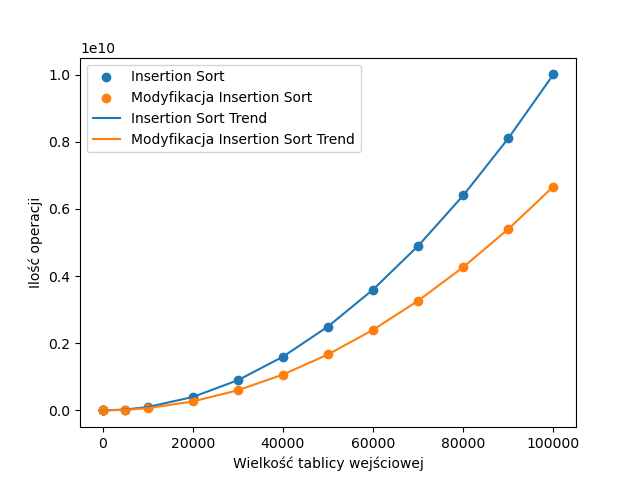
\includegraphics[width=0.8\textwidth]{Figure_1.png}
    \caption{Ilość operacji w zależności od rozmiarów tablicy wejściowej}
    \label{fig:insertion}
\end{figure}
\subsection{Merge Sort}
\textit{Merge Sort} to algorytm sortowania działający w czasie \( \Theta(n \log n) \). Poniżej przedstawiamy kluczowy fragment jego implementacji:
\begin{lstlisting}[style=mystyle, language=C++, caption={Implementacja Merge Sort}, label={lst:mergesort}]
void merge_sort(float A[], int p, int k)
{
  if (p < k)
  {
    int s = p + (k - p) / 2;
    merge_sort(A, p, s);
    merge_sort(A, s + 1, k);
    merge(A, p, s, k);
  }
}
\end{lstlisting}
Algorytm działa poprzez rekurencyjne dzielenie tablicy na dwie podtablice aż do momentu, gdy każda z nich ma tylko jeden element. Takie tablice jednoelementowe są naturalnie posortowane. Następnie następuje proces łączenia dwóch posortowanych podtablic w jedną większą.

Funkcja \texttt{merge}, odpowiedzialna za łączenie posortowanych podtablic, jest zdefiniowana w następujący sposób:

\newpage
 
\begin{lstlisting}[style=mystyle, language=C++, caption={Implementacja Merge}, label={lst:merge}]
void merge(float A[], int p, int s, int k)
{
  int n1 = s - p + 1;
  int n2 = k - s;
  float L[n1 + 1];
  float R[n2 + 1];
  L[n1] = numeric_limits<float>::infinity();
  R[n2] = numeric_limits<float>::infinity();
  for (int i = 0; i < n1; ++i)
  {
    L[i] = A[i + p];
  }
  for (int j = 0; j < n2; ++j)
  {
    R[j] = A[j + s + 1];
  }
  int i = 0;
  int j = 0;
  for (int l = p; l <= k; ++l)
  {
    if (L[i] <= R[j])
    {
      A[l] = L[i];
      ++i;
    }
    else
    {
      A[l] = R[j];
      ++j;
    }
  }
} 
\end{lstlisting}
Funkcja \texttt{merge} przypisuje elementy z tablicy \( A[p \ldots s] \) do tablicy \( L \) oraz elementy z tablicy \( A[s+1 \ldots k] \) do tablicy \( R \). Następnie iteruje przez tablice \( L \) i \( R \), wybierając za każdym razem mniejszy element i wstawiając go w odpowiednie miejsce w tablicy \( A \). Na wyjściu otrzymujemy posortowaną tablicę, składającą się z elementów \( A[p \ldots s] \) i \( A[s+1 \ldots k] \).
\subsubsection{Modyfikacja Merge Sort}
W tej modyfikacji algorytm dzieli tablicę na trzy części zamiast dwóch. Kluczowe różnice w implementacji tego algorytmu w porównaniu do oryginalnej wersji obejmuje dodanie nowych miejsc podziału oraz dodanie dodatkowego rekurencyjnego wywołania w funkcji \texttt{merge\_sort}:

\begin{lstlisting}[style=mystyle, language=C++, caption={Fragment implementacji modyfikacji Merge Sort}, label={lst:mergesort2}]
int s1 = p + (k - p) / 3;
int s2 = p + 2 * ((k - p) / 3);
merge_sort(A, p, s1);
merge_sort(A, s1 + 1, s2);
merge_sort(A, s2 + 1, k);
merge(A, p, s1, s2, k);
\end{lstlisting}

Dodatkowo w funkcji \texttt{merge} wprowadzamy nową tablicę \( M \):
\begin{lstlisting}[style=mystyle, language=C++, caption={Fragment implementacji modyfikacji Merge}, label={lst:merge2}]
float M[n2 + 1];
\end{lstlisting}

Działanie zmienionej funkcji jest analogiczne do oryginalnej, z tą różnicą, że łączenie odbywa się teraz dla trzech tablic zamiast dwóch:
\begin{lstlisting}[style=mystyle, language=C++, caption={Fragment implementacji modyfikacji Merge}, label={lst:merge2l}]
int i = 0;
int j = 0;
int z = 0;

for (int l = p; l <= k; ++l)
{
    if (L[i] <= R[j] && L[i] <= M[z])
    {
        A[l] = L[i];
        ++i;
    }
    else if (M[z] <= R[j] && M[z] <= L[i])
    {
        A[l] = M[z];
        ++z;
    }
    else
    {
        A[l] = R[j];
        ++j;
    }
}
\end{lstlisting}
Ilość operacji wykonywanych przez modyfikację algorytmu Merge możemy opisać poprzez rekurencyjne równanie:
\[
    T(n) = 3T(n/3) + n
\]
Możemy zatem zapisać:
\[
    T(n) = \sum_{k=0}^{\log_3 n} 3^k\left(\frac{n}{3^k}\right) = n\sum_{k=0}^{\log_3 n} 1 = \Theta(n \log n)
\]
Intuicyjnie, dzięki szybszemu przejściu do zbiorów jednoelementowych, modyfikacja powinna być bardziej efektywny od orginału.
\subsubsection{Wyniki dla Merge Sort}
Tabele poniżej przedstawiają wyniki eksperymentów dla algorytmu Merge Sort oraz jego modyfikacji na tablicach o różnej wielkości:
\begin{table}[H]
    \centering
    \begin{tabular}{|c|c|c|c|}
    \hline
    \textbf{Wielkość tablicy} & \textbf{Ilość przypisań} & \textbf{Ilość porównań} & \textbf{Łączna liczba operacji} \\ \hline
    5 & 108 & 57 & 165 \\ \hline
    10 & 278 & 148 & 426 \\ \hline
    100 & 4,548 & 2,512 & 7,060 \\ \hline
    5,000 & 369,028 & 210,420 & 579,448 \\ \hline
    10,000 & 788,068 & 450,844 & 1,238,912 \\ \hline
    50,000 & 4,522,308 & 2,603,388 & 7,125,696 \\ \hline
    80,000 & 7,504,628 & 4,326,780 & 11,831,408 \\ \hline
    100,000 & 9,544,628 & 5,506,780 & 15,051,408 \\ \hline
    \end{tabular}
    \caption{Liczba operacji dla algorytmu Merge Sort przy różnych rozmiarach tablicy}
    \label{tab:merge_results}
\end{table}

\begin{table}[H]
    \centering
    \begin{tabular}{|c|c|c|c|}
    \hline
    \textbf{Wielkość tablicy} & \textbf{Ilość przypisań} & \textbf{Ilość porównań} & \textbf{Łączna liczba operacji} \\ \hline
    5 & 99 & 67 & 166 \\ \hline
    10 & 256 & 180 & 436 \\ \hline
    100 & 3,560 & 2,791 & 6,351 \\ \hline
    5,000 & 277,738 & 234,773 & 512,511 \\ \hline
    10,000 & 555,727 & 481,819 & 1,037,546 \\ \hline
    50,000 & 3,318,096 & 2,880,715 & 6,198,811 \\ \hline
    80,000 & 5,238,096 & 4,635,715 & 9,873,811 \\ \hline
    100,000 & 6,706,625 & 5,931,401 & 12,638,026 \\ \hline
    \end{tabular}
    \caption{Liczba operacji dla modyfikacji algorytmu Merge Sort przy różnych rozmiarach tablicy}
    \label{tab:m_merge_results}
\end{table}

Z tabel wynika, że modyfikacja algorytmu Merge Sort jest bardziej wydajna dla większych tablic. Różnice te są dobrze zobrazowane na Wykresie \ref{fig:merge}.

\begin{figure}[H]
    \centering
    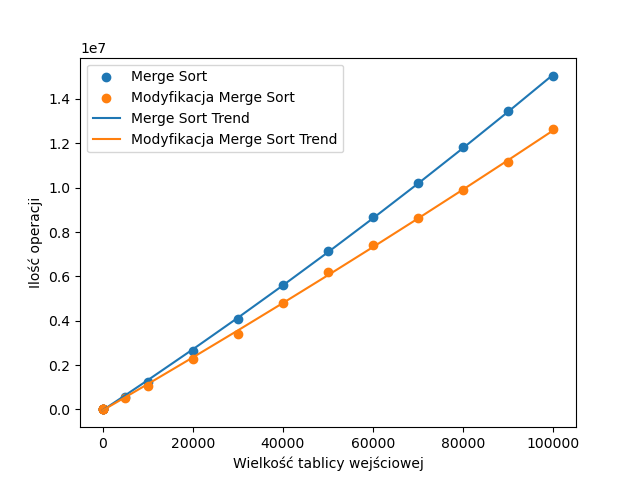
\includegraphics[width=0.8\textwidth]{Figure_2.png}
    \caption{Ilość operacji w zależności od rozmiarów tablicy wejściowej}
    \label{fig:merge}
\end{figure}
\subsection{Heap Sort}
\textit{Heap Sort} to algorytm sortowania działający w czasie \( \bigO (n \log n) \). Poniżej przedstawiamy kluczowy fragment jego implementacji:
\begin{lstlisting}[style=mystyle, language=C++, caption={Implementacja Heap Sort}, label={lst:heapsort}]
void heap_sort(heap &A, int n)
{
  build_heap(A, n);
  for (int i = n - 1; i > 0; --i)
  {
    float temp = A[i];
    A[i] = A[0];
    A[0] = temp;
    --A.heap_size;
    heapify(A, 0);
  }
}
\end{lstlisting}
Algorytm jest oparty na strukturze kopca binarnego (dokładniej, na kopcu typu maksymalnego), czyli drzewie binarnym, w którym wartość każdego węzła jest mniejsza niż wartość jego rodzica(własność \textbf{MAX\_HEAP}). W naszej implementacji kopiec jest reprezentowany jako tablica, wraz z dodatkowym parametrem \textbf{heap\_size}, który przechowuje aktualny rozmiar kopca:

\newpage

\begin{lstlisting}[style=mystyle, language=C++, caption={Implementacja Heap}, label={lst:heap}]
struct heap
{
  float *array;
  int heap_size = 0;

  float &operator[](int idx)
  {
    return array[idx];
  }
  heap(float *arr)
  {
    array = arr;
  }
};
\end{lstlisting}
Dodatkowo definiujemy dwie funkcje \textbf{left} oraz \textbf{right} zwracające lewe i prawe dziecko węzła o indeksie \( i \):
\begin{lstlisting}[style=mystyle, language=C++, caption={Implementacja Left i Right}, label={lst:lr}]
int left(int i)
{
  return 2 * i + 1;
}

int right(int i)
{
  return 2 * i + 2;
}
\end{lstlisting}
Definiujemy również funkcję \textbf{heapify}, która rekurencyjnie naprawia własność \textbf{MAX\_HEAP} dla węzła o indeksie \( i \), pod warunkiem, że poddrzewa o wierzchołkach będących dziećmi węzła o indeksie \( i \) mają już własność \textbf{MAX\_HEAP}. Funkcja działa poprzez zamianę węzła z dzieckiem o największej wartości, jeśli jest to konieczne:
\begin{lstlisting}[style=mystyle, language=C++, caption={Implementacja Heapify}, label={lst:heapify}]
void heapify(heap &A, int i)
{
  int l = left(i);
  int r = right(i);
  int largest = i;
  if (l < A.heap_size && A[l] > A[i]) {
    largest = l;
  }
  if (r < A.heap_size && A[r] > A[largest]) {
    largest = r;
  }
  if (i != largest)
  {
    float temp = A[i];
    A[i] = A[largest];
    A[largest] = temp;
    heapify(A, largest);
  }
}
\end{lstlisting}
Algorytm działa poprzez zbudowanie kopca z tablicy \textbf{A} przy pomocy funkcji \textbf{build\_heap}, która wywołuje funkcję \textbf{heapify} dla każdego węzła, który nie jest liściem:

\begin{lstlisting}[style=mystyle, language=C++, caption={Implementacja Build Heap}, label={lst:buildheap}]
void build_heap(heap &A, int n)
{
  A.heap_size = n;
  for (int i = (n / 2); i >= 0; --i)
  {
    heapify(A, i);
  }
}
\end{lstlisting}

Następnie, algorytm iteracyjnie zamienia wierzchołek (największy element) z ostatnim liściem (węzłem o największym indeksie), wywołuje funkcję \textbf{heapify} na wierzchołku oraz zmniejsza parametr \textbf{heap\_size} o jeden. Po zakończeniu pętli \textbf{for} otrzymujemy posortowaną tablicę \textbf{A}.
\subsubsection{Modyfikacja Heap Sort}
W tej modyfikacji algorytm używa kopców trenarnych zamiast binarnych. Kluczowe różnice w implementacji tego algorytmu w porównaniu do oryginalnej wersji obejmuje dodanie funkcji \textbf{MID}, która zwraca środkowe dziecko węzła, oraz zmiana kodu funkcji \textbf{LEFT} i \textbf{RIGHT}:
\begin{lstlisting}[style=mystyle, language=C++, caption={Implementacja Left, Mid i Right}, label={lst:lmr}]
int left(int i)
{
  return 3 * i + 1;
}

int mid(int i)
{
  return 3 * i + 2;
}

int right(int i)
{
  return 3 * i + 3;
  ;
}
\end{lstlisting}
Dodatkowo, w funkcji \textbf{HEAPIFY} wybieramy największe dziecko z trzech zamiast dwóch:
\begin{lstlisting}[style=mystyle, language=C++, caption={Część implementacji zmodyfikowanego Heapify}, label={lst:buildheap2}]
  int l = left(i);
  int m = mid(i);
  int r = right(i);
  if (l < A.heap_size && A[l] > A[i])
  {
    largest = l;
  }
  comparisions += 2;
  if (m < A.heap_size && A[m] > A[largest])
  {
    largest = m;
  }
  comparisions += 2;
  if (r < A.heap_size && A[r] > A[largest])
  {
    largest = r;
  }
\end{lstlisting}
Reszta kodu pozostaje analogiczna. Dzięki posiadaniu większej liczby liści w kopcu trenarnym, efektywność modyfikacji algorytmu powinna być wyższa.

\textbf{BUILD\_HEAP} działa w czasie \( \bigO(n) \), zatem zmodyfikowany algorytm działa w czasie \( \bigO (n \log n) \).

\subsubsection{Wyniki dla Heap Sort}
Tabele poniżej przedstawiają wyniki eksperymentów dla algorytmu Heap Sort oraz jego modyfikacji na tablicach o różnej wielkości:
\begin{table}[H]
    \centering
    \begin{tabular}{|c|c|c|c|}
    \hline
    \textbf{Wielkość tablicy} & \textbf{Ilość przypisań} & \textbf{Ilość porównań} & \textbf{Łączna liczba operacji} \\ \hline
    5 & 85 & 70 & 155 \\ \hline
    10 & 232 & 183 & 415 \\ \hline
    100 & 4,562 & 3,308 & 7,870 \\ \hline
    5,000 & 438,290 & 305,525 & 743,815 \\ \hline
    10,000 & 951,673 & 661,035 & 1,612,708 \\ \hline
    50,000 & 5,631,385 & 3,887,342 & 9,518,727 \\ \hline
    80,000 & 9,412,168 & 6,487,715 & 15,899,883 \\ \hline
    100,000 & 12,012,335 & 8,274,443 & 20,286,778 \\ \hline
    \end{tabular}
    \caption{Liczba operacji dla algorytmu Heap Sort przy różnych rozmiarach tablicy}
    \label{tab:heap_results}
\end{table}

\begin{table}[H]
    \centering
    \begin{tabular}{|c|c|c|c|}
    \hline
    \textbf{Wielkość tablicy} & \textbf{Ilość przypisań} & \textbf{Ilość porównań} & \textbf{Łączna liczba operacji} \\ \hline
    5 & 83 & 78 & 161 \\ \hline
    10 & 211 & 195 & 406 \\ \hline
    100 & 3,803 & 3,290 & 7,093 \\ \hline
    5,000 & 347,976 & 289,958 & 637,934 \\ \hline
    10,000 & 749,096 & 621,005 & 1,370,101 \\ \hline
    50,000 & 4,405,541 & 3,633,093 & 8,038,634 \\ \hline
    80,000 & 7,338,882 & 6,037,845 & 13,376,727 \\ \hline
    100,000 & 9,348,531 & 7,686,258 & 17,034,789 \\ \hline
    \end{tabular}
    \caption{Liczba operacji dla modyfikacji algorytmu Heap Sort przy różnych rozmiarach tablicy}
    \label{tab:m_heap_results}
\end{table}

Z tabel wynika, że modyfikacja algorytmu Heap Sort jest bardziej wydajna dla większych tablic. Różnice te są dobrze zobrazowane na Wykresie \ref{fig:heap}.

\begin{figure}[H]
    \centering
    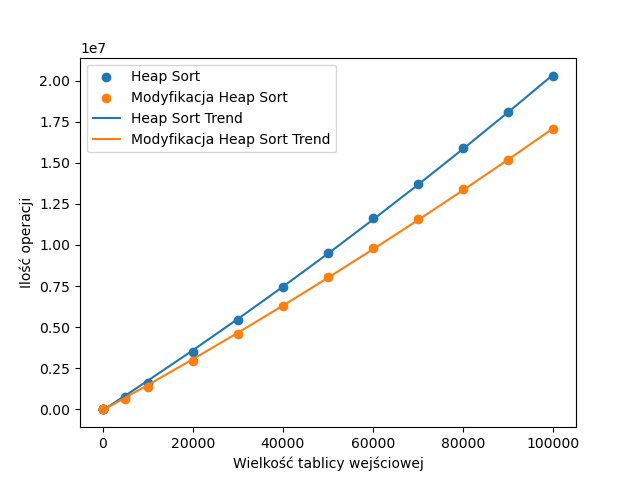
\includegraphics[width=0.8\textwidth]{Figure_3.png}
    \caption{Ilość operacji w zależności od rozmiarów tablicy wejściowej}
    \label{fig:heap}
\end{figure}
\section{Wnioski}
Na podstawie przeprowadzonej analizy algorytmów, \textit{Insertion Sort} może być wydajny dla niewielkich zestawów danych, jednak w miarę zwiększania się rozmiaru tablicy liczba wykonywanych operacji rośnie nawet o trzy rzędy wielkości w porównaniu do \textit{Merge Sort} i \textit{Heap Sort}.

Porównując \textit{Merge Sort} i \textit{Heap Sort} możemy zauważyć, że pierwszy z nich jest zauważalnie szybszy:
\begin{figure}[H]
    \centering
    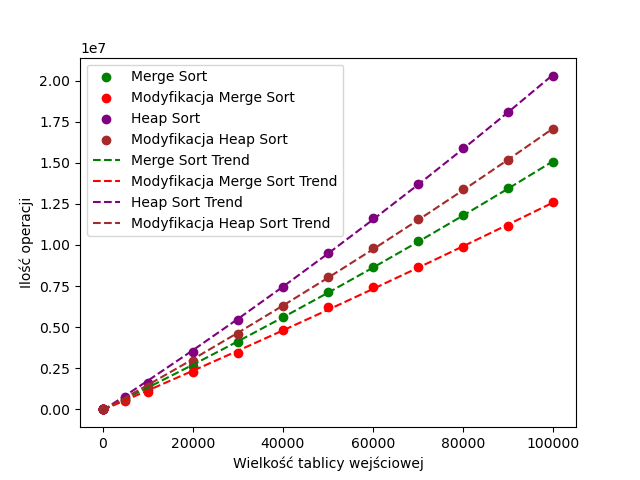
\includegraphics[width=0.8\textwidth]{Figure_4.png}
    \caption{Ilość operacji w zależności od rozmiaru tablicy wejściowej}
    \label{fig:heapmerge}
\end{figure}
Jednak \textit{Merge Sort} posiada jedną znaczącą wadę – złożoność pamięciową. Z powodu konieczności definiowania dodatkowych tablic \textbf{L} i \textbf{R}, ilość pamięci potrzebnej do działania algorytmu jest nieporównywalnie większa niż w przypadku \textit{Heap Sort}. Wybór odpowiedniego algorytmu zależy więc od dostępnych zasobów.

Zaproponowane modyfikacje algorytmów okazują się bardziej efektywne od ich oryginałów; różnica jest szczególnie widoczna w przypadku dużych zestawów danych. Warto zatem rozważyć ich zastosowanie, zwłaszcza gdy zasoby są mocno ograniczone.
\end{document}